\section{E3: Changing the model}
\renewcommand{\Ex}{E3}
Up to this point, all experiments have employed the observation and state space models outlined in the introduction of the Experiments section (see \ref{sec:experiments}). However, using these models in scenarios presented by videos \textit{V1, V2, V3} comes with several disadvantages. The state space model assumes uniform position uncertainty in all directions for targets. Additionally, the videos are not captured from a bird's-eye view but from an angled perspective. This camera angle causes detected targets to appear smaller when they are farther away and larger when they are closer to the camera. Consequently, this effect alters the actual movement model of the targets, which our current model does not account for.


Considering the videos utilized in this study, we can leverage prior knowledge regarding potential targets, such as cars, movement patterns. It is established that cars are inclined to move in the direction of the road rather than backwards or sideways.
\subsection{V2}
\renewcommand{\Vs}{V2}
For this experiment video \textit{V2} with the added crossing road as an obstacle is used. The video is observed at the rate 14 fps.

The state space CVM model is employed with transition matrix

\begin{align}
    F_k &=
    \begin{bmatrix}
        1 & 0 & 2*\Delta & 0\\
        0 & 1 & 0 & \Delta \\
        0 & 0 & 1.1 & 0 \\
        0 & 0 & 0 & 1.1
    \end{bmatrix}

\end{align}
and process covariance matrix
\begin{align}
    Q_k &=
    \begin{bmatrix}
        2 & 0.5 & 0 & 0\\
        0 & 1 & 0 & \Delta \\
        0 & 0 & 1 & 0 \\
        0 & 0 & 0 & 1
    \end{bmatrix}
    * 0.003,
    \label{eq:exp_E3-V2_Q}
\end{align}
where $\Delta = 1$
The observation covariance matrix is reformulated as
\begin{align}
    R_k &=
    \begin{bmatrix}
        2 & 0.5 \\
        0 & 1
    \end{bmatrix}
    * 20.
    \label{eq:exp_E3-V2_R}
\end{align}

The spawning point providing nearby targets with initial covariance matrix $P$ is established as
\begin{align}
    P_k &=
    \begin{bmatrix}
        80 & 20 & 0 & 0 \\
        0 & 40 & 0 & 0 \\
        0 & 0 & 40 & 0 \\
        0 & 0 & 0 & 40
    \end{bmatrix}. \label{eq:exp_E3-V2_P}
\end{align}

These model formulations ensure that the noise covariance takes an ellipsoidal shape rather than a circular one. These ellipses are oriented in the direction of the road, indicating that uncertainty increases more in alignment with the road's direction. This implies a lower probability of a car being positioned next to the road in the subsequent time step.
\subsection{V2b -- GM-PHD with dynamic detection probability}
The GM-PHD filter with the dynamic detection probability is analysed only in this experiment. The best performing settings are used - \textit{S3}, i.e., grounded SAM.

\subsubsection{S3 -- Grounded SAM}
\renewcommand{\Set}{S3}
Note in Table \ref{tab:\Ex-\Vs-\Set}, that the standard pruning threshold $T_p$ is the same as the lowered pruning threshold $T_l$. Due to the better model settings and dynamic detection probability, it is not neccesarry to lower the pruning threshold for targets in \textit{detected} and \textit{hidden} state.
\begin{table}[H]
    \centering
    \begin{tabular}{|c|c|c|c|c|c|c|c|c|c|}
        \hline
        $P_{D,k}(x)$ & $P$ & $\sigma_{\upsilon}$ & $\sigma_{\epsilon}$ & $T_H$ & $T_d$ & $T_p$ & $T_l$ & $T_{text}$ & $T_{bbox}$\\ \noalign{\hrule
        height 1.5pt}
        0.3 & see \ref{eq:exp_E3-V2_P} & see \ref{eq:exp_E3-V2_Q} & see \ref{eq:exp_E3-V2_R} & 0.6 & 3 & 0.1 & 0.1 & 0.3 & 0.3\\
        \hline
    \end{tabular}
    \caption{The parameter settings for experiment {\Ex-\Vs-\Set} with dynamic detection probability.}
    \label{tab:\Ex-\Vs-\Set}
\end{table}

In Figure \ref{fig:\Ex-\Vs-\Set} we can see the tracking performance of the GM-PHD filter with settings \textit{S1} on traffic situation with an added obstacle.
\begin{itemize}
    \item \textbf{\ref{fig:\Ex-\Vs-\Set:01}:} This sequence starts with frame no. 44. Due to the targets' close postions, more than 2 targets appears in the place where only two true targets are present.
    \item \textbf{\ref{fig:\Ex-\Vs-\Set:02}:} The targets enter under the obstacle.
    \item \textbf{\ref{fig:\Ex-\Vs-\Set:03}:} The first frame with misdetected objects. The targets are already in \textit{hidden state}.
    \item \textbf{\ref{fig:\Ex-\Vs-\Set:04}:} The targets' predicted positions are already behind the true targets' positions.
    \item \textbf{\ref{fig:\Ex-\Vs-\Set:05}:} As the predicted covariance grows, the targets merged into a single one. The cars are clearly seen, but the YOLO model does not detect them.
    \item \textbf{\ref{fig:\Ex-\Vs-\Set:06}:} The cars are detected and initialized by the target. The predicted black bounding box still interfers with the added obstacle, thus the target is considered as hidden.
    \item \textbf{\ref{fig:\Ex-\Vs-\Set:07}:} In this frame, the predicted black bounding box moves to the area with natural traffic line. The false target is in \textit{dead} state and is removed immediately.
    \item \textbf{\ref{fig:\Ex-\Vs-\Set:08}:} The targets continue in their paths with correct positions.
\end{itemize}

In this experiment, we have demonstrated, that if an obstacle differs from the targets' background scene, the pruning given by the Markov process works exceptionally well. The downside of this approaches lies in additional settings of further parameters.
\begin{figure}[H]
    \centering
    \begin{subfigure}{\textwidth}
        \centering
        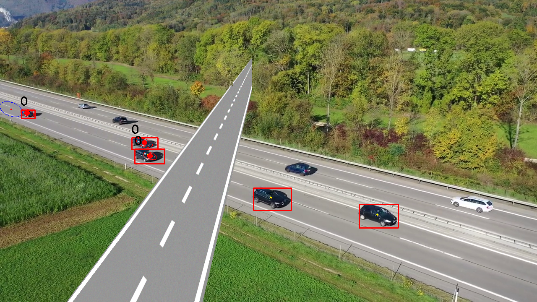
\includegraphics[width=0.85\linewidth]{../../../experiments/\Ex/\Vs/DINO/44}
        \caption{Frame number: 44.}
        \label{fig:\Ex-\Vs-\Set:01}
    \end{subfigure}
    \begin{subfigure}{\textwidth}
        \centering
        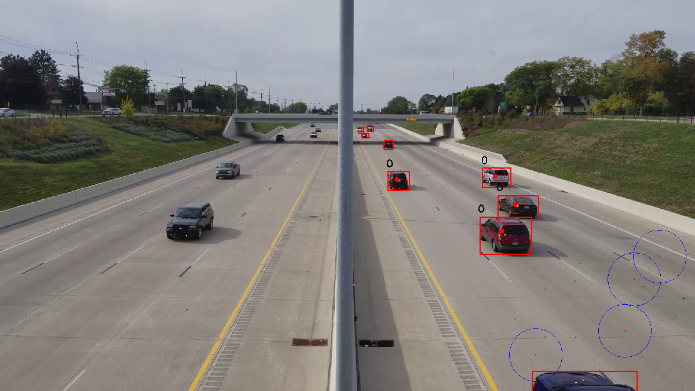
\includegraphics[width=0.85\linewidth]{../../../experiments/\Ex/\Vs/DINO/48}
        \caption{Frame number: 48.}
        \label{fig:\Ex-\Vs-\Set:02}
    \end{subfigure}
    \\
    \begin{subfigure}{\textwidth}
        \centering
        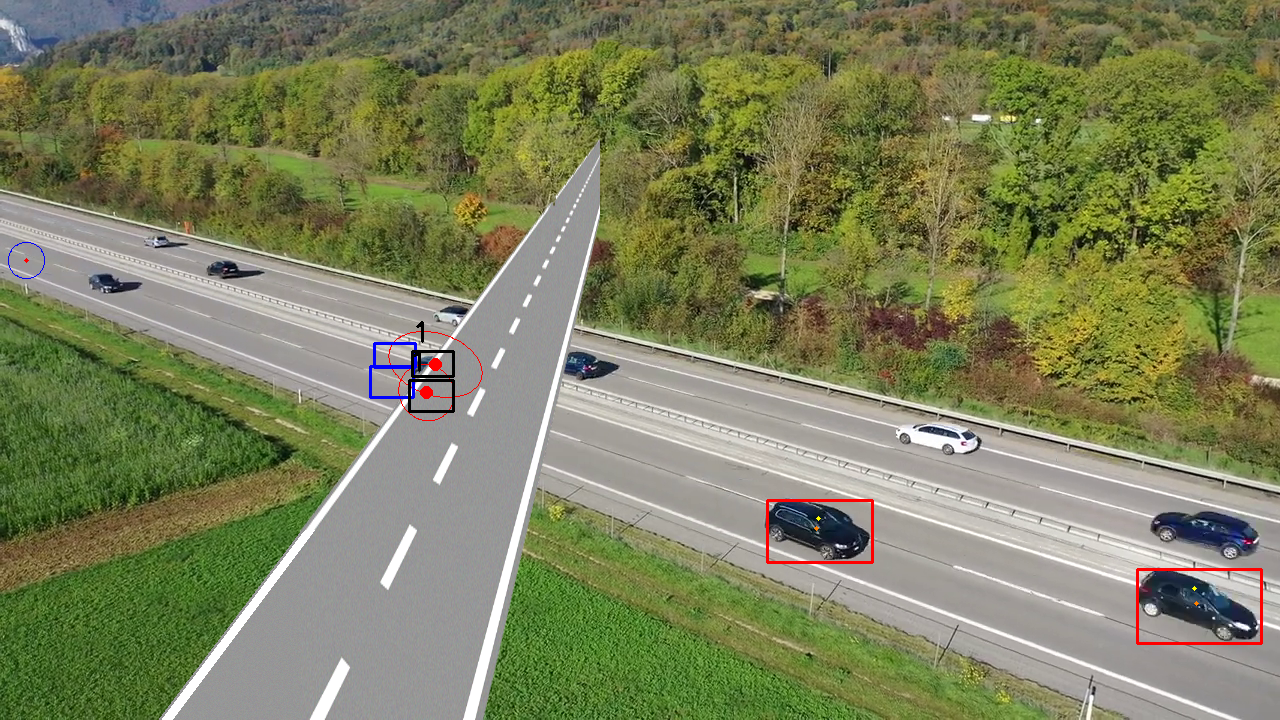
\includegraphics[width=0.85\linewidth]{../../../experiments/\Ex/\Vs/DINO/50}
        \caption{Frame number: 50.}
        \label{fig:\Ex-\Vs-\Set:03}
    \end{subfigure}
    \caption{Image sequence of tracked objects using GM-PHD filter with dynamic detection probability, Grounded SAM and adjusted models -- part 1.}
    \label{fig:\Ex-\Vs-\Set_1}
\end{figure}
\begin{figure}[H]

    \begin{subfigure}{\textwidth}
        \centering
        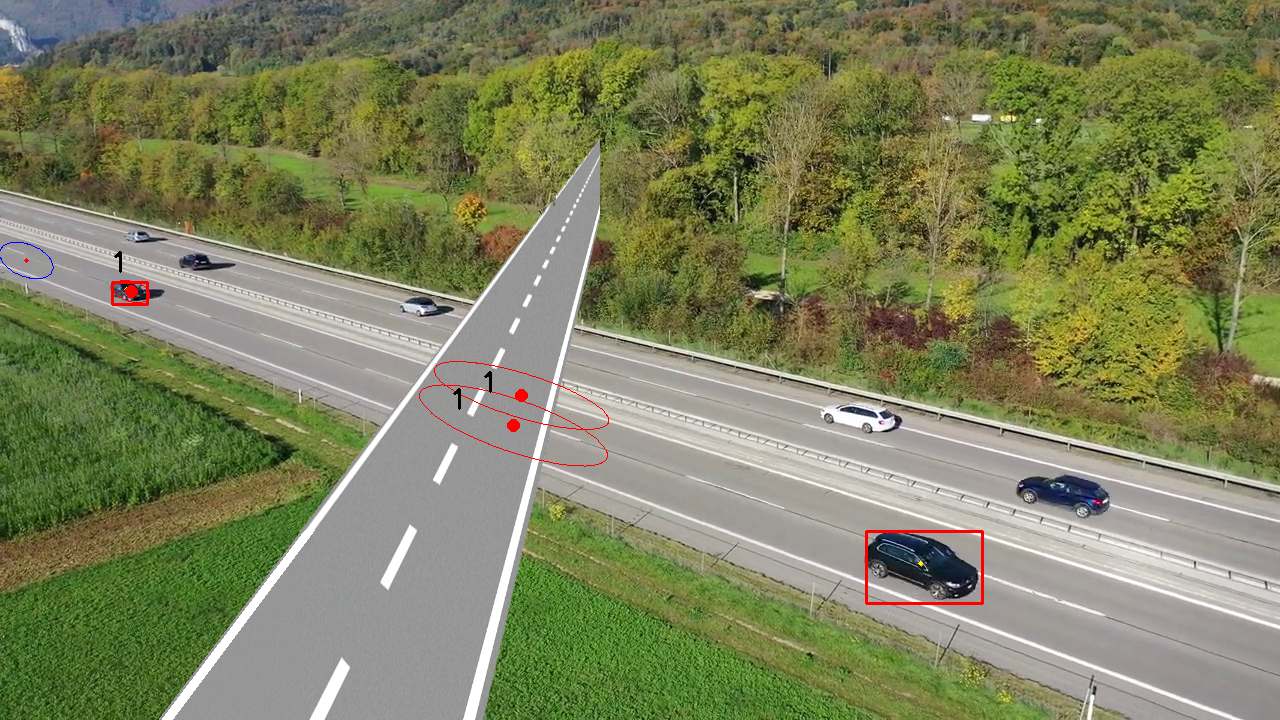
\includegraphics[width=0.85\linewidth]{../../../experiments/\Ex/\Vs/DINO/53}
        \caption{Frame number: 53.}
        \label{fig:\Ex-\Vs-\Set:04}
    \end{subfigure}
    \\
    \begin{subfigure}{\textwidth}
        \centering
        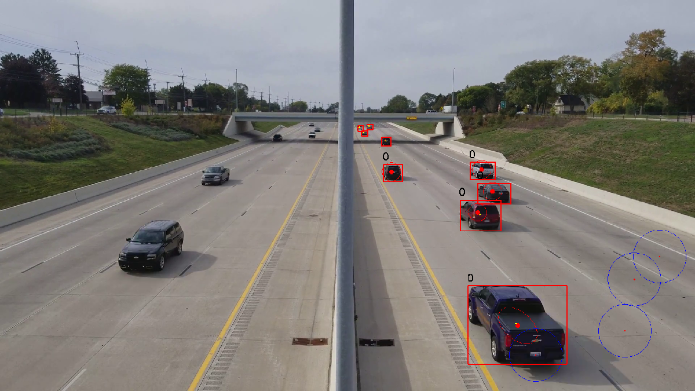
\includegraphics[width=0.85\linewidth]{../../../experiments/\Ex/\Vs/DINO/54}
        \caption{Frame number: 54.}
        \label{fig:\Ex-\Vs-\Set:05}
    \end{subfigure}
    \begin{subfigure}{\textwidth}
        \centering
        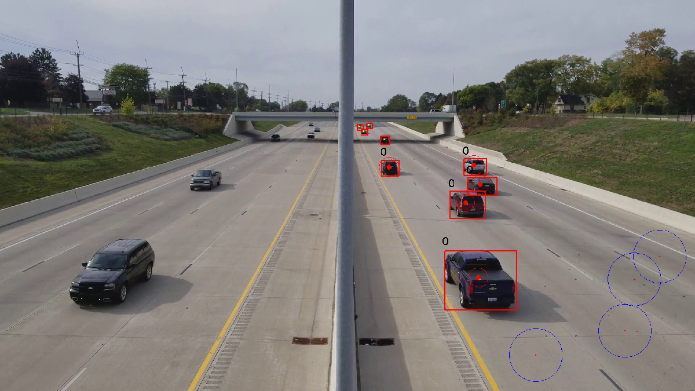
\includegraphics[width=0.85\linewidth]{../../../experiments/\Ex/\Vs/DINO/58}
        \caption{Frame number: 58.}
        \label{fig:\Ex-\Vs-\Set:06}
    \end{subfigure}
    \caption{Image sequence of tracked objects using GM-PHD filter with dynamic detection probability, Grounded SAM and adjusted models -- part 2.}
    \label{fig:\Ex-\Vs-\Set_2}
\end{figure}

